\documentclass[tikz,border=0pt]{standalone}
\usepackage[utf8]{inputenc}
\usepackage{csquotes}
\usepackage{xcolor}
\usepackage{graphicx}
\usepackage{pgffor}
\usepackage{listings}
\usepackage{array}
\usepackage{fontawesome}
\usepackage{amsmath}

\lstset{
    basicstyle=\ttfamily\fontsize{6}{8}\selectfont,
    breaklines=true,
    % backgroundcolor=\color{black},
    keywordstyle=\color{pink},
    commentstyle=\color{blue},
    stringstyle=\color{white},
    showstringspaces=false,
    frame=none,
    xleftmargin=0.6cm,
    xrightmargin=0.6cm
}

\begin{document}
\begin{tikzpicture}
\useasboundingbox (0,0) rectangle (10.8,10.8);

% Hintergrund in Schwarz
\fill[black] (0,0) rectangle (10.8,10.8);

% Zufällige Einsen und Nullen verteilen
\foreach \i in {1,...,5000} {
    \node[text=green, opacity=0.1, font=\ttfamily\fontsize{5}{6}\selectfont] at (rand*10.8, rand*10.8) {\pgfmathtruncatemacro{\random}{round(rand)}\random};
}

% \fill[red, opacity=0.1] (0.05,5.95) rectangle (10.75,10.75);
% \draw[red, thin] (0.05,5.95) rectangle (10.75,10.75); % 45% Höhe
\node[red, anchor=north west, font=\ttfamily\bfseries\fontsize{8}{9}\selectfont] at (0.1,10.65) {NVD DB Update {\Large{ CVE-2025-0108} - \textbf{Score:}{\Large{ 9.1 }}}};
% % ------------------------------------------------------------------------------------------------------------------------------
% \node[red, anchor=north west, font=\ttfamily\fontsize{8}{9}\selectfont, text width=10.6cm, align=center] at (0.1,10.25) {
% \newline
% \newline
% \newline
% If you want to succeed in penetration testing and cybersecurity, learn at least:
% \newline
% };
% ------------------------------------------------------------------------------------------------------------------------------
\fill[green, opacity=0.1] (0.05,1.15) rectangle (10.75,10.75);
\draw[green, thin] (0.05,1.15) rectangle (10.75,10.75); % 45% Höhe
% \node[green, anchor=north west, font=\ttfamily\bfseries\fontsize{8}{9}\selectfont] at (0.1,5.65) {Solution:};
% ------------------------------------------------------------------------------------------------------------------------------
\node[green, anchor=north west, font=\ttfamily\fontsize{8}{9}\selectfont, text width=10.6cm, align=center] at (0.1,10.25) {
\textbf{Components:}
\begin{scriptsize}
\begin{lstlisting}
 paloaltonetworks pan-os *
 paloaltonetworks pan-os 10.2.9
 paloaltonetworks pan-os 10.2.8
 paloaltonetworks pan-os 10.2.7
 paloaltonetworks pan-os 11.2.4
 paloaltonetworks pan-os 10.2.13
 paloaltonetworks pan-os 10.2.12
 paloaltonetworks pan-os 11.1.6
 paloaltonetworks pan-os 10.1.14
\end{lstlisting}
\end{scriptsize}
\textbf{Description:}
\begin{scriptsize}
\begin{lstlisting}
An authentication bypass in the Palo Alto Networks PAN-OS software enables an unauthenticated attacker with network access to the management web interface to bypass the authentication otherwise required by the PAN-OS management web interface and invoke certain PHP scripts. While invoking these PHP scripts does not enable remote code execution, it can negatively impact integrity and confidentiality of PAN-OS. You can greatly reduce the risk of this issue by restricting access to the management web interface to only trusted internal IP addresses according to our recommended best practices deployment guidelines https://live.paloaltonetworks.com/t5/community-blogs/tips-amp-tricks-how-to-secure-the-management-access-of-your-palo/ba-p/464431 . This issue does not affect Cloud NGFW or Prisma Access software.
\end{lstlisting}
\end{scriptsize}
\textbf{Main problems:}
\begin{scriptsize}
\begin{lstlisting}
306 "Missing Authentication for Critical Function"

\end{lstlisting}
\end{scriptsize}
};
% ------------------------------------------------------------------------------------------------------------------------------
\draw[green, thin] (0.05,0.05) rectangle (10.75,1.05); % 10% Höhe
% \node[green, anchor=north west, font=\ttfamily\bfseries\fontsize{5}{6}\selectfont] at (0.1,0.95) {Contact:};

% Tabelle 2x2 im Contact Block
\node[green, anchor=north west, font=\ttfamily\fontsize{8}{9}\selectfont, text width=10.6cm] at (0.1,0.95) {
\begin{tabular}{@{}p{4.8cm}@{}p{5cm}@{}}
\faGlobe\ https://cybersword.tech & \faLinkedin\ www.linkedin.com/in/cybersword-tech \\
\faInstagram\ ph1sher & \faTwitter\ @davidwowa \\
\end{tabular}
};
\end{tikzpicture}
\end{document}